\documentclass[11pt,a4paper]{article}
\usepackage[T1]{fontenc}
\usepackage[ngerman]{babel}
\usepackage{amsmath}
\usepackage{parskip}
\usepackage{graphicx}
\usepackage{listings}
\usepackage{hyperref}
\usepackage{float}

%opening
\author{Simon Cholewa}
\title{7. Tool Supported Data Cleaning}

\hyphenation{
	Mo-tor-ü-ber-wach-ung 
}


\begin{document}

\maketitle

\section{dsm-beuth-edl-demodata-dirty}

\textit{Clean the \hyperref{https://raw.githubusercontent.com/edlich/eternalrepo/master/DS-WAHLFACH/dsm-beuth-edl-demodata-dirty.csv}{}{}{dsm-beuth-edl-demodata-dirty.csv} mini csv from the first exercise with Trifacta Wrangler (if you have no cloud access use the download version).}

\textit{Not the red bars that give you instant feedback (on big datasets) where errors could be!}

\textit{Create a recipie to clean the data as good as you can (it must not be a general script). Try to upload only one file (e.g. with screenshots and the end result). (10 points)}

\begin{figure}[H]
	\centering
	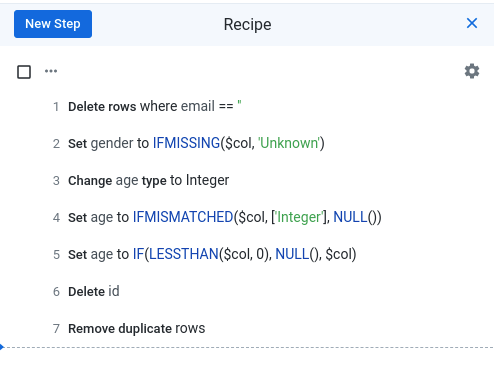
\includegraphics[width=0.8\linewidth]{images/recipe}
	\caption[Das Rezept]{Das Rezept}
	\label{fig:recipe}
\end{figure}

\begin{figure}[H]
	\centering
	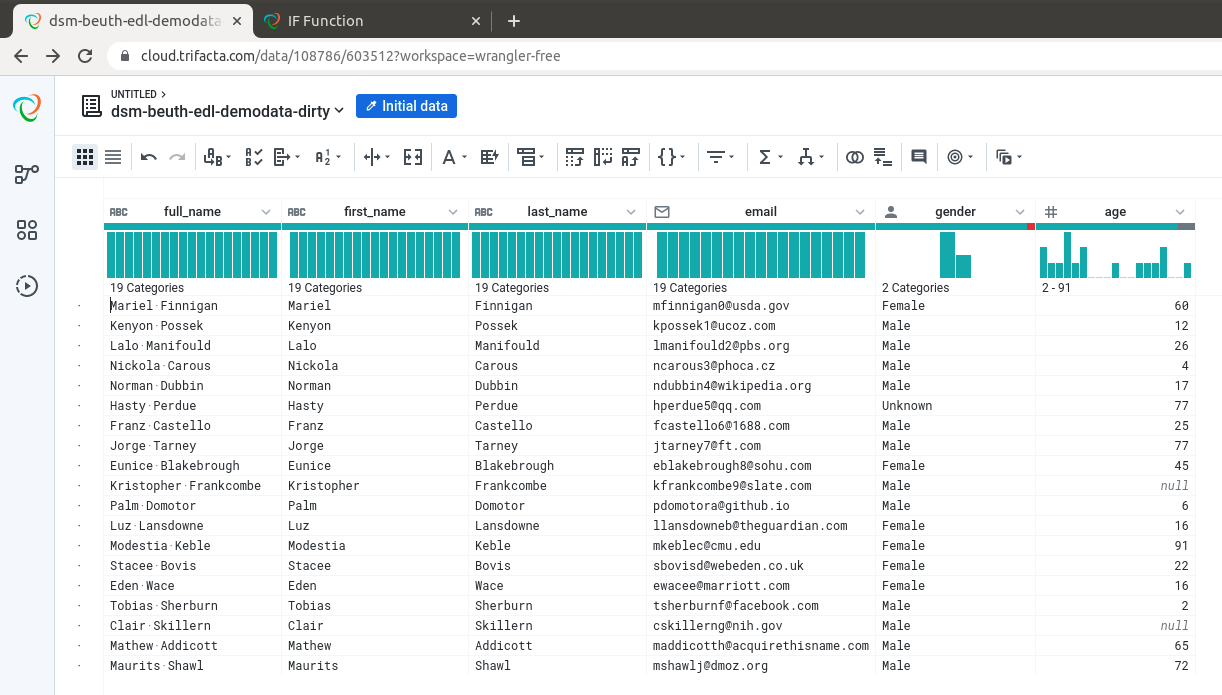
\includegraphics[width=1\linewidth]{images/wrangled_data}
	\caption[Die verarbeiteten Daten]{Die verarbeiteten Daten}
	\label{fig:wrangleddata}
\end{figure}



\section{15 Years of Power Outages}

\textit{Load\ the\ Grid\_Disruption\_00\_14\_standardized -}\\ \textit{Grid\_Disruption\_00\_14\_standardized.csv Dataset from Kaggle:
\hyperref{https://www.kaggle.com/autunno/15-years-of-power-outages}{}{}{15 YEARS OF POWER OUTAGES}.}

\textit{Where are errors here? => Describe some errors and a possible cleaning in text.}

In der Spalte \textit{Time Event Began} existieren 23 Einträge, die von Trifcata nicht korrekt zugeordnet werden können, darunter fehlende Werte, die mit ,,NA'' (oder einmal mit ,,N/A'')gekennzeichnet sind. Andere Werte sind beispielsweise ,,Midnight'' oder ,,Evening'', bei anderen fehlt ein Punkt (,,p.m'') oder es wurden zu viele Punkte oder Leerzeichen genutzt.

Aufgrund der geringen Anzahl an Werten, kann hier manuell nachgebessert werden. Fehlende Werte sollten (automatisch) durch \textit{null} ersetzt werden.

Weiteres Eingreifen ist in der Spalte ,,Date of Restoration'' erforderlich. Hier finden sich neben den Daten Einträge wie ,,NA'', ,,Unknown'' und ,,Ongoing''. Diese Werte könnten auch mit \textit{null} bewertet werden, da sie nicht seriös durch konkrete Werte ersetzt werden könnten. Hier handelt es sich um 33 betroffene Werte.

Die Spalte ,,Time of Restoration'' verhält sich ähnlich, allerdings finden sich hier einige Werte, die automatisch korrigiert werden könnten, da ein anderes Zeitformat genutzt wurde (mit Angabe von Sekunden und ,,PM'' statt ,,p.m.''). Bei wenigen Werten wurde auch ein Punkt vergessen (,,a.m'').

Die korrigierbaren Fehler sollten korrigiert werden. Fehlende Werte in den Zeit- und Datumsspalten treten gehäuft auf, insbesondere bei ,,Date of Restoration'' und ,,Time of Restoration'' (s. Abb. \ref{fig:recipetimerestoration}). Daher sollte in Anbetracht der großen Datenmenge (1652) auch Löschen der betroffenen Datensätze erwogen werden. Somit erspart man sich später sicherlich Probleme und der Informationsverlust ist gering.

Die größte Herausforderung stellen die Spalten ,,Demand Loss (MW)'' (s. Abb. \ref{fig:recipedemandloss}) und ,,Number of Customers Affected'' (s. Abb. \ref{fig:recipenumaffectedcustomers}) dar, denn der Anteil der fehlenden Werte ist größer. Weiterhin wurden die existierenden Zahlenwerte in verschiedenen Formaten hinterlegt.

\textit{How would you clean this file? (5 Points) => Try to create some cleaning recipies in Trifacta (e.g. 3) The idea here is that I can see, you have dug into this system! You must not clean all errors.}

\begin{figure}
	\centering
	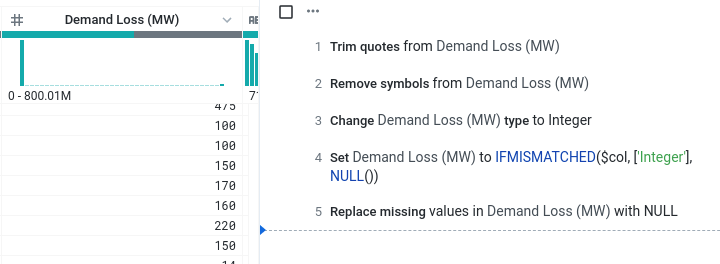
\includegraphics[width=1\linewidth]{images/recipe_Demand_Loss}
	\caption[Demand Loss]{Rezept für die Spalte ,,Demand Loss (MW)''}
	\label{fig:recipedemandloss}
\end{figure}

\begin{figure}
	\centering
	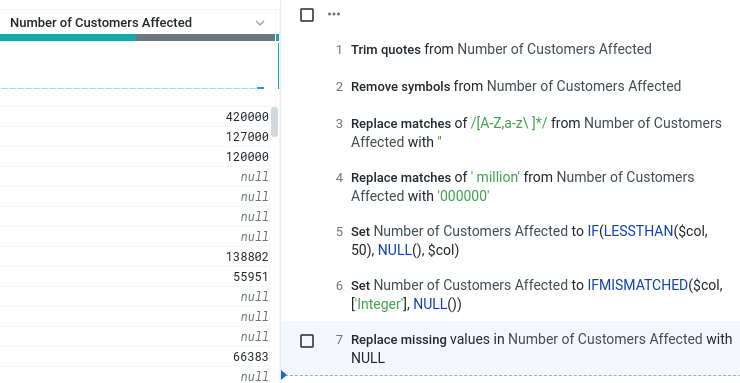
\includegraphics[width=1\linewidth]{images/Recipe_NumAffectedCustomers}
	\caption[Number of Customers Affected]{Rezept für die Spalte ,,Number of Customers Affected''}
	\label{fig:recipenumaffectedcustomers}
\end{figure}

\begin{figure}
	\centering
	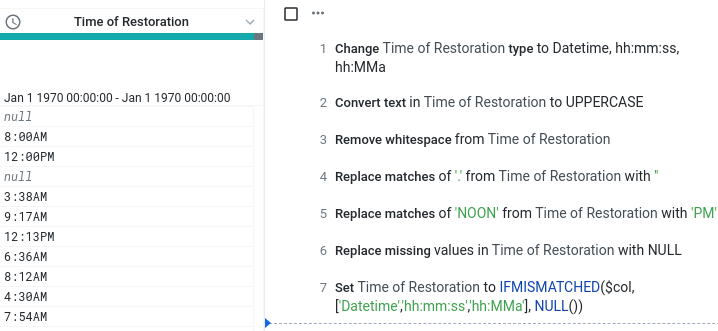
\includegraphics[width=1\linewidth]{images/recipe_TimeRestoration}
	\caption[Time of Restoration]{Rezept für die Spalte ,,Time of Restoration''}
	\label{fig:recipetimerestoration}
\end{figure}


\end{document}
